% arara: pdflatex: { shell: yes }
% arara: biber 
% arara: pdflatex: { shell: yes }
% arara: pdflatex: { shell: yes }



\pdfminorversion=7  % see https://www.overleaf.com/learn/latex/%5Cpdfminorversion and https://www.overleaf.com/learn/latex/%5Cpdfinclusionerrorlevel
                    % and the answer in https://tex.stackexchange.com/questions/542343/epstopdf-pdfminorversion-7-error


\documentclass[a4paper, 12pt, oneside]{book}

%-----------------------------------------------------------------------------
% Packages
%-----------------------------------------------------------------------------
\usepackage[T1]{fontenc}            % Font encoding
\usepackage[utf8]{inputenc}         % Input encoding
\usepackage[english,italian]{babel} % Text Language (secondaria, primaria)
\usepackage[babel]{csquotes}        % Dipendenza di babel
\usepackage{microtype}              % Improves text writing
\usepackage[backend=biber,autolang=hyphen]{biblatex}% Imports biblatex package
\setcounter{biburlnumpenalty}{9000}
\setcounter{biburlucpenalty}{9000}
\setcounter{biburllcpenalty}{9000}
\addbibresource{./BackMatter/Tesi.bib}% Import the bibliography file
\usepackage{standalone}
\usepackage{graphicx}               % Required for inserting images
\graphicspath{ {./Images/} }        % Folder path to images. Path relative to the main .tex file  
\usepackage{subfig}
\usepackage{caption}
\captionsetup{format=hang,labelfont=bf}
\usepackage{float}                  % For figures
% \usepackage[x11names]{xcolor}
\usepackage{xcolor}
\usepackage{fancyhdr}               % For the headings      
\usepackage{listings}               % Uso dei listing per il codice
\usepackage{svg}
\usepackage{lipsum}                 % Dummy package
\usepackage{afterpage}
\usepackage[most]{tcolorbox}
% \tcbuselibrary{breakable}
\usepackage{tikz}
\usetikzlibrary{mindmap,shadows}
\usepackage{shapepar}
\usepackage{titlesec}
\usepackage{comment}
\usepackage[font={itshape,small}]{quoting}
\quotingsetup{font=small}
\usepackage{mathtools} % loads also amsmath package
\usepackage{amssymb}
\usepackage{amsfonts} % for \mathbb
\usepackage{amsthm}
\usepackage{bm}  % for accessing bold math symbols
\usepackage{cancel}
\usepackage{booktabs} % for tables
\usepackage{algorithm}
\usepackage{algpseudocode}  %load automatically the algorithmicx package
\usepackage{customization} % IMport custom preamble 
\usepackage[hidelinks]{hyperref}
% \usepackage{minted} % for language highlight
% \usemintedstyle{friendly}
\hypersetup{
    pdfstartview = XYZ null null 1.00,  % open the generated pdf with 100% zoom by default
    pdftitle={Tesi}, 
}


%-----------------------------------------------------------------------------
% Document Start
%-----------------------------------------------------------------------------
\begin{document}

\frontmatter
%-------------------------------------------------------------------------
%\begin{titlepage}

\thispagestyle{empty}

\begin{center}
    \Large{UNIVERSITÀ DEGLI STUDI DI \\ CASSINO E DEL LAZIO MERIDIONALE}
\end{center}

%---------------------
% Unicas_Emblem 
%---------------------
\begin{figure}[!htp]
    \centering
    
\includegraphics[keepaspectratio=true,scale=0.25]{images/Frontespizio/Unicas_logo.pdf}
\end{figure}

\begin{center}
    \normalsize{DIPARTIMENTO DI INGEGNERIA ELETTRICA \\ E DELL'INFORMAZIONE “MAURIZIO SCARANO”}
    \vspace{4mm}
    \\ \normalsize{CORSO DI LAUREA IN INGEGNERIA INFORMATICA \\ E DELLE TELECOMUNICAZIONI}
\end{center}


\vspace{7mm}


\begin{center}
    \LARGE{\textbf{ Assessment delle performance di Elixir nell'ambito IOT.\\ }}
\end{center}


\vspace{20mm}


\begin{minipage}[t]{0.47\textwidth}
	{\normalsize{\textbf{Relatore:}}{\normalsize\vspace{3mm}
	\\ \large{Prof. Ciro D'Elia}}}
\end{minipage}
\hfill
\begin{minipage}[t]{0.47\textwidth}\raggedleft
	{\normalsize{\textbf{Candidato:}}{\normalsize\vspace{3mm} 
        \\ \large{Nico Fiorini}}}
\end{minipage}


\vspace{30mm}


{\centering{\large{ANNO ACCADEMICO 2022/2023}}\par}



%\end{titlepage}


\cleardoublepage
    \thispagestyle{empty}
        \vspace*{\stretch{1}}
		{\large
            \begin{flushright}
				Ai miei nonni,\\
				che hanno contribuito\\
				a plasmare la persona che sono oggi.
				\vspace{2em}

				There's a lot of beauty in the ordinary things.\\
				\textit{The Office - Pam Beesly}

            \end{flushright}
        \vspace{\stretch{2}}
		}
\cleardoublepage
\afterpage{\null\thispagestyle{empty}\clearpage}
 
\begingroup 
\titleformat{\chapter}
{\normalfont\Huge\bfseries\centering} %shape
%{\centering} % format
{}% label
{} % sep
{}  

\chapter*{Abstract}

L'industria del software è attualmente alle prese con
la crescente esigenza di sviluppare applicazioni
sempre più scalabili e performanti per gestire efficacemente
l'aumento del numero di utenti e dei servizi
che utilizzano tali applicazioni.
In particolare, nel contesto dell'Internet of Things (IoT),
un settore in costante sviluppo, la reattività,
la tolleranza agli errori e la scalabilità emergono
come fattori cruciali.

In questo contesto, Elixir, un linguaggio di programmazione 
funzionale e concorrente basato su Erlang, emerge come una 
scelta promettente per la costruzione di sistemi altamente 
affidabili e reattivi, nonché la sua capacità di
gestire carichi di lavoro intensivi e flussi di dati in
tempo reale tipici delle applicazioni IoT.

Questo studio si propone di analizzare le caratteristiche 
di Elixir che lo rendono un linguaggio degno di nota,
e attraverso una serie di esperimenti empirici si misurano le
performance di Elixir, anche mettendolo a confronto con altre
soluzioni più diffuse.

I risultati di questa ricerca forniscono una base per valutare
l'efficacia di Elixir, contribuendo così alla comprensione del
ruolo che questo linguaggio può svolgere nel futuro dello
sviluppo delle applicazioni IoT.

\endgroup

% s\include{}

\tableofcontents % Prints the main table of contents

%-------------------------------------------------------------------------
\mainmatter

% Introduzione
\chapter{Introduzione}

Elixir è un linguaggio di programmazione dinamico e funzionale
sviluppato nel 2012 da José Valim,
con l'obbiettivo di favorire una maggiore scalabilità
e produttività nella macchinia virtuale di Erlang,
mantenendo al contempo la compatibilità con l'ecosistema
di Erlang\cite{Elixirpr12:online}.
Elixir si è affermato come una promettente scelta
nell'industria del software,specialmente in contesti dove è
richiesta scalabilità, tolleranza agli errori e reattività 
grazie al suo approccio concorrenziale.


In particolare, Elixir può risultare vantaggioso nel campo dell'IoT per diversi motivi:
\begin{enumerate}
	\item \textbf{Concorrenza}: Nell'ambito dell'IoT, la gestione simultanea
	di dispositivi è essenziale. Elixir, grazie alla sua capacità 
	di gestire facilmente la concorrenza, consente il monitoraggio
	e il controllo efficiente di numerosi dispositivi contemporaneamente.
	\item \textbf{Fault Tolerance}: 
	Data la natura degli ambienti IoT, dove i dispositivi possono
	guastarsi improvvisamente, Elixir offre strumenti per la supervisione
	e la gestione degli errori, garantendo la continuità delle operazioni
	anche in caso di fallimenti.
	\item \textbf{Sviluppo Rapido e Manutenzione}:
	Elixir è un linguaggio moderno che offre una sintassi efficiente e snella,
	oltre a strumenti di sviluppo come Mix per la gestione delle dipendenze
	e l'ambiente interattivo iex. La presenza di un package manager (Hex)\cite{Hex63:online}
	e la possibilità di generare automaticamente la documentazione
	facilitano il processo di sviluppo e manutenzione del codice.
	
\end{enumerate}

Il trattato esplora Elixir concentrandosi su due aspetti principali:
la semplicità e le performance. Si analizzano i punti di forza di 
un linguaggio funzionale e come questi sono sfruttati in Elixir, con 
un focus sulla concorrenza. Nella scelta di un linguaggio, la semplicità
è fondamentale e deve essere accessibile a tutti i programmatori.
Tuttavia, l'efficienza è altrettanto importante, quindi vengono condotti
test empirici per valutare le performance di Elixir.

In particolare il lavoro effettuato è così ripartito: 


\begin{itemize}
	\item Nel capitolo 2 si discute del linguaggio funzionale,
	esaminando le astrazioni offerte da Elixir per lo svilluppo
	di codice affidabile, si tratta la concorrenza e come la Erlang VM
	si occupa della gestione dei processi.
	% TODO migliorare
	\item Nel capitolo 3 si spiega il lavoro sperimentale svolto e i risultati
	ottenuti (continuare)

\end{itemize}




% Capitolo 1
\chapter{Caratteristiche di Elixir}\label{chap:Caratteristiche}

\section{Introduzione}



In questo capitolo, esamineremo le caratteristiche distintive
di Elixir, un linguaggio di programmazione funzionale e
concorrente che sfrutta appieno la potenza della piattaforma
OTP (Open Telecom Platform).

Elixir, scritto in Erlang e eseguito sulla macchina virtuale
Erlang (BEAM), eredita gli obiettivi di Erlang, ma apporta
miglioramenti significativi per rendere il linguaggio più
appetibile e moderno.

Erlang, nato nel 1986, è stato progettato per semplificare
lo sviluppo di software concorrente e robusto.
Elixir si basa su queste fondamenta solide, offrendo un'API
più pulita e astrazioni avanzate che consentono ai programmatori
di ragionare a un livello più elevato, facilitando la scrittura
di codice concorrente in modo intuitivo.

Una delle massime principali di Erlang e, di conseguenza,
di Elixir, è "Let it crash" (Lascia che si schianti),
che riflette l'approccio alla gestione degli errori nei sistemi
concorrenti, incoraggiando la gestione degli errori tramite
il rilancio e la supervisione anziché il blocco del processo.

Per capire come lavorare con questo linguaggio, bisogna affrontare
un po' di questioni e farsi un po' di domande.
Bisogna capire come la macchina virtuale Beam affronta la concorrenza,
Elixir in particolare è un linguaggio orientato alla concorrenza e 
le astrazioni che fornisce sono proprio per far sì che
si programmi in modo concorrenziale portando ad avere un
codice responsivo e gestendo bene i processi attraverso 
il meccanismo di Supervision, il software diventa anche robusto.
Un altro punto da affrontare è l'immutabilità dei dati, è un concetto
chiave in Elixir ed Erlang, è proprio questa caratteristica
che ci semplifica la programmazione concorrenziale.

\section{Il paradigma funzionale}
\renewcommand\lstlistingname{Esempio}
Come già accennato Elixir è un linguaggio funzionale, dove
il concetto di funzione ricopre il ruolo di protagonista,
i dati sono immutabili e il codice è dichiarativo.

Questo modo di vedere le cose deriva dal Lambda calcolo o $\lambda$-calcolo
\cite{Lambdaca75:online}
un sistema formale definito da Alonzo Church nel 1936, sviluppato
per definire formalmente le funzioni e il loro calcolo.

In un paradigma basato su stati come la programmazione ad oggetti
spesso si hanno variabili condivise mutabili, ovvero, più parti del codice
possono riferirsi alla stessa variabile, e questo complica la programmazione
multithreading dovendosi preoccupare di meccanismi come il blocco
sincronizzato o il locking per evitare le race condition tra più parti
del codice, e non è immediato scrivere del codice concorrenziale sicuro
e spesso si riscontrano comportamenti indeterminati.
In un paradigma funzionale si predilogono le variabili immutabili che
aggirano questo problema riducendo il rischio di scrivere codice
concorrenziale non sicuro.

Cambiare paradigma non è immediato, un paradigma si può dire che
definisce il modo di pensare al problema, nella programmazione ad
oggetti per esempio si definiscono le cosidette classi,
pensando al problema come oggetti che possono comportarsi in un
determinato modo attraverso le funzioni definite su di esso.
Perciò si pensa ad un oggetto che ha un comportamento e che cambia
il suo stato nel tempo, un modo di sviluppare intuitivo ma non sempre
ottimale per la risoluzione di problemi. Nella programmazione funzionale
si cambia prospettiva, ovvero si ha un input, si passa l'input 
alla funzione e si ottiene la trasformazione dell'input ottenendo
l'output.

In poche parole un linguaggio funzionale assume che scrivere un
software complesso sia più facile nel momento in cui il codice ha
queste proprietà:
\begin{itemize}
    \item I dati sono immutabili
    \item Le funzioni sono pure, ovvero, il risultato di una funzione
    dipende soltanto dai suoi parametri in input.
    \item Le funzioni non generano effetti oltre il suo valore restituito.
\end{itemize}

Con queste proprietà si ha più controllo del flusso del programma,
anche se non sempre possono essere soddisfatte.

%------------------------------------------------------------------

\subsection{Struttura di un progetto Elixir}

Elixir è un linguaggio moderno, e come ogni linguaggio moderno che
si rispetti fornisce un tool per la creazione e configurazione di
progetti, questo tool si chiama \textbf{Mix}.

%------------------------------------------------------------------

\subsubsection{Il tool Mix}
È possibile creare un progetto con il comando:

\begin{lstlisting}[language=none]
mix new <nome-progetto>
\end{lstlisting}

Verrà creata una struttura per il progetto come nell'esempio \ref{lst:struttura_progetto},
il codice sarà organizzato nella cartella \textbf{lib}, viene creata una
cartella \textbf{test}, e il file per la configurazione del progetto \textbf{mix.exs}.
Da notare che anche la configurazione del progetto avviene tramite funzioni.

\begin{lstlisting}[language=none,captionpos=b,caption={Struttura progetto},label={lst:struttura_progetto}]
.
>build
>deps
  -->...
>lib
  -->example.ex
mix.exs
README.md
>test
  -->example.exs
\end{lstlisting}

Come sappiamo Elixir fornisce anche un ambiente interattivo (\textbf{iex}) per
testare il nostro codice, ed è consentito avviare questo ambiente nel
dominio della nostra applicazione con il comando:

\begin{lstlisting}[language=none]
iex -S mix 
\end{lstlisting}
Si può compilare il progetto con:
\begin{lstlisting}[language=none]
mix compile
\end{lstlisting}

Con Mix possiamo includere e scaricare facilmente anche librerie esterne attraverso
il package manager.\cite{HexDocs99:online}

\subsubsection{Moduli}
Elixir organizza il codice in Moduli, permettendo di definire
le funzioni dentro dei namespace, così da separare
le responsabilità delle funzioni.

Ci sono varie cose che si possono definire dentro un modulo,
si possono definire delle \textbf{struct}
ma cosa più importante si possono definire i cosiddetti 
\textbf{Behaviour}, un modo per definire un interfaccia Api,
Elixir fornisce delle astrazioni proprio attraverso questi.
%TODO menzionare GenServer e Supervisor
Ciò che si vuole evidenziare ora è che il progetto è definito
in moduli, il modo che Elixir fornisce per organizzare il
codice.

% ----------------------------------------------------------------------------

\subsection{Basi dichiarative}

Come già accennato, Elixir adotta un approccio
dichiarativo nella definizione delle funzioni.
Questo si contrappone all'approccio imperativo,
che si concentra su "come posso risolvere questo problema?",
mentre quello dichiarativo si pone la domanda 
"come posso definire un problema?".

Nell'esempio \ref{lst:somma_n_cpp} è presentato un approccio
imperativo al problema "somma dei primi n elementi", mentre
nell'esempio \ref{lst:somma_n_elixir} è presentato l' approccio dichiarativo
con Elixir.


\begin{lstlisting}[language=cpp, caption={Somma N elementi},captionpos=b,
	label={lst:somma_n_cpp}]
int sum_first_n(n){
  int sum=0;
    for(int i=1;i++;i<=n){
      sum+=i;
    }
    return sum;
}
\end{lstlisting}

\begin{lstlisting}[language=elixir, caption={Somma N elementi},captionpos=b,
	label={lst:somma_n_elixir}]
defmodule Sum do
  def sum_recursive(0), do: 0
  def sum_recursive(n), do: n + sum_recursive(n - 1)
end
\end{lstlisting}

In particolare questo approccio è rafforzato tramite il meccanismo
del \textbf{Pattern Matching}, infatti in Elixir l'operatore $=$,
non è un operatore di assegnazione, ma è comparabile
all'equivalente algebrico.
Quest'operatore ci permette di scrivere dell'equazioni
che condizionano il flusso del codice.
Questo è molto utile per l'approccio
dichiarativo, infatti possiamo definire più corpi della stessa funzione
ed Elixir capisce quale funzione invocare in base
al valore dei suoi parametri attraverso questo meccanismo,
è già stato utilizzato implicitamente nell'esempio \ref{lst:somma_n_elixir},
dove viene invocata la funzione "sum\_recursive(0)" quando
il valore dell'argomento vale 0, altrimenti chiamerà quello
con l'argomento "n" assegnando il valore dell'argomento alla variabile n.

Elixir cerca di assegnare il valore a destra dell'equazione
al valore di sinistra cercando di risolvere l'equazione tentando
di fare un assegnazione dove possibile.
Questo ci permette di usare quest'operatore per poter
scomporre un dato, un esempio può essere usato usando l'ambiente
interattivo \textit{iex}

\begin{lstlisting}[language=elixir, caption={Pattern Matching},captionpos=b,
	label={lst:pattern_matching}]
# Lists
iex> list = [1, 2, 3]
[1, 2, 3]
iex> [1, 2, 3] = list
[1, 2, 3]
iex> [] = list
** (MatchError) no match of right hand side value: [1, 2, 3]
iex> [1 | tail] = list
[1,2,3]
iex> tail
[2,3]
\end{lstlisting}

%--------------------------------------------------------------------------

\subsection{Transizione al funzionale - Immutabilità dei dati}

Cambiare paradigma può essere difficoltoso, bisogna
cambiare prospettiva, ma con le giuste intuizioni
può risultare semplice. Per fare una transizione al funzionale
bisogna capire soprattuto qual'è la differenza rispetto ad un
linguaggio basato sugli stati.

Elixir non ha oggetti, il linguaggio ha un forte focus sull'immutabilità.
In Elixir trasformiamo dati piuttosto che mutarli, infatti da questo
punto di vista probabilmente è più naturale il paradigma funzionale
piuttosto che un procedurale, ad esempio in un linguaggio
procedurale possiamo scrivere:

\begin{lstlisting}[language=cpp]
my_array = [1,2,3]
do_something_with_array(my_array)
print(my_array)
\end{lstlisting}

Ci potremmo aspettare che la stampa dell'array sia [1,2,3] quando in realtà
l'output dipende da cosa fa la funzione. Mentre in Elixir questa cosa
non è implicita, ma l'assegnazione deve essere sempre esplicita come
segue:

\begin{lstlisting}[language=elixir]
my_list = [1,2,3]
my_list = do_something_with_array(my_list)
IO.inspect(my_list)
\end{lstlisting}

Se my\_list non viene riassegnata, my\_list non cambia.
Il problema può arrivare nel momento in cui ci serve uno stato
da condividere, una semplice variabile globale non esiste
in Elixir, e per mantenere uno stato dobbiamo
affidarci ad un altro processo che lo mantiene per noi,
ed Elixir almeno per questo ci da delle astrazioni
a cui fare affidamento come il Modulo \textbf{Agent} o il
\textbf{GenServer} che verranno trattati in seguito.

%--------------------------------------------------------------------------
\subsection{Conseguenze sulle prestazioni dell'immutabilità}

L'immutabilità ci consente di avere un controllo maggiore
sul flusso del codice, questo però può portare ad un'inefficienza
dovendo sempre copiare dati, inoltre si può pensare che si creano
molti dati non più utilizzati da liberare in memoria con il Garbage collector.
Sfruttando questa proprietà però si possono limitare i danni.

Elixir sa che i dati sono immutabili, e può riusarli in parte o per
intero quando si creano nuove strutture.
Il seguente esempio mostra come Elixir ottimizza la creazione di
nuovi dati:

\begin{lstlisting}[language=elixir]
iex> lista1 = [ 3, 2, 1 ]
[3, 2, 1]
iex> lista2 = [ 4 | lista1 ]
[4, 3, 2, 1]
\end{lstlisting}

La lista2 infatti è creata usando la lista1 sapendo che non
cambierà mai durante il flusso di esecuzione, quindi mette
semplicimente in coda la lista1.

\subsubsection{Garbage Collection}
Un altro aspetto che può creare dubbi sul copiare dati, è che
si lasciano spesso vecchi dati non più utilizzati da dover
pulire con il Garbage Collector.

Scrivendo codice Elixir però ci rendiamo subito conto
che ci porta a sviluppare codice con migliaia di processi leggeri,
ed ogni processo ha il proprio heap. I dati nell'applicazione quindi
sono suddivisi nei processi, e ogni heap è molto piccolo rendendo
il garbage collector molto veloce. Se un processo termina prima che
il suo heap diventi pieno, tutti i suoi dati vengono eliminati, senza necessità
di liberare la memoria rendendo il garbage collector
efficiente. \cite{programming_elixir_immutability}


\section{Concorrenza}

La concorrenza è un concetto fondamentale nell'ambito
dello sviluppo software, si riferisce alla capacità
di eseguire più attività contemporaneamente.
Questo è particolarmente importante in applicazione
che devono gestire molteplici operazioni in parallelo
come ad esempio un server web, applicazioni di
elaborazione dati e sistemi real time.

La concorrenza consente a un programma di sfruttare appieno
le risorse disponibili, e migliorando
la responsività di un programma.
Inoltre, permette di creare sistemi più reattivi e
scalabili, in grado di gestire un numero crescente di
richieste senza compromettere le prestazioni.

In generale, la gestione della concorrenza in molti linguaggi
può essere complessa
e soggetta a errori o comportamenti indeterminati, infatti,
più processi o thread possono interagire tra loro in modo
imprevedibile, essendo così costretti a usare tecniche di
locking in concomitanza di memoria condivisa trà più thread.

Nel contesto di Elixir, la concorrenza è un concetto centrale
e viene gestita attraverso il modello di programmazione
basato su processi leggeri, tutti isolati tra loro con il proprio
stack ed il proprio heap.

% ------------------------------------------------------

\subsection{La concorrenza in Beam}

La concorrenza gioca un ruolo chiave per un software
che vuole essere altamente responsivo.
La piattaforma Erlang fa uso dei cosiddetti processi leggeri,
non sono processi del 
sistema operativo, ma processi della
VM Beam, chiamato processo e non thread in quanto non
condividono memoria e sono completamente
isolati tra di loro a differenza dei thread.

Un server tipico deve gestire migliaia di richieste, e
gestirle concorrenzialmente è essenziale per non far
rimanere in attesa il client. Quello che si vuole è
gestirli parallelamente il più possibile sfruttando
più risorse della Cpu disponibile.
Quello che fa la macchina virtuale per noi è permetterci
la scalabilità, più richieste allora più risorse da allocare.

Inoltre, siccome il processo è isolato, un errore in una richiesta
può essere localizzato senza avere impatto
sul resto del sistema, così creando anche un sistema robusto
agli errori.

Un processo appena creato occupa in memoria 326 words \cite{ErlangPr21:online},
quindi in una macchina a 64 bit occupa 2608 byte.
Lo si può vedere in Elixir facilmente con l'esempio \ref{lst:memoryoneprocess}.

\begin{lstlisting}[language=elixir, caption={Memoria in un processo},captionpos=b,
	label={lst:memoryoneprocess}]
defmodule Examples.Memory do
  def mypid do
    receive do
      :stop -> :exit
      _ -> mypid()
    end
  end
 
  def benchmark do
    pid = spawn(fn -> mypid() end)
    {_,byte_used} = :erlang.process_info(pid,:memory)
    IO.puts("La memoria usata dal processo e': #{byte_used} byte")
    send pid, :stop
  end
end
\end{lstlisting}

Infatti l'output ottenuto dall'esempio \ref{lst:memoryoneprocess} è:
\begin{lstlisting}[language=none]
iex> Examples.Memory.benchmark
La memoria usata dal processo e': 2640 byte
:stop
\end{lstlisting}
	
Si nota dall'output dell'esempio che la memoria utilizzata
è leggermente superiore della memoria minima dichiarata,
infatti il processo non fa nulla di particolare oltre
ad aspettare il messaggio di ":stop".
È da notare che è proprio questa leggerezza nei processi che
permette al linguaggio di essere orientato alla concorrenza,
permettendo di usare i processi senza troppe remure. 

Un altro punto da notare è che si può migliorare significativamente
la reattività del programma ma non l'efficienza totale del
sistema, infatti non tutti i processi
sono eseguiti in parallelo, quindi in una macchina con quattro
processori non si possono eseguire più di 4 processi per volta
ed in un normale software Elixir è normale avere migliaia di
processi che lavorano, lavorando con migliaia di processi
però permette di distribuire il delay di operazioni concorrenti.

Facendo un esempio con una Cpu dual-core,
i processi vengono eseguiti concorrenzialmente e gestiti
dagli Scheduler della VM,
in figura \ref{fig:concorrenza_beam} è mostrato come
la VM gestisce i processi, la VM è un unico processo
nel sistema operativo e alloca uno scheduler per ogni
core logico disponibile sulla macchina, gli scheduler si
occupano di gestire l'esecuzione dei processi uno per volta.

\begin{figure}[!htp]
    \centering
    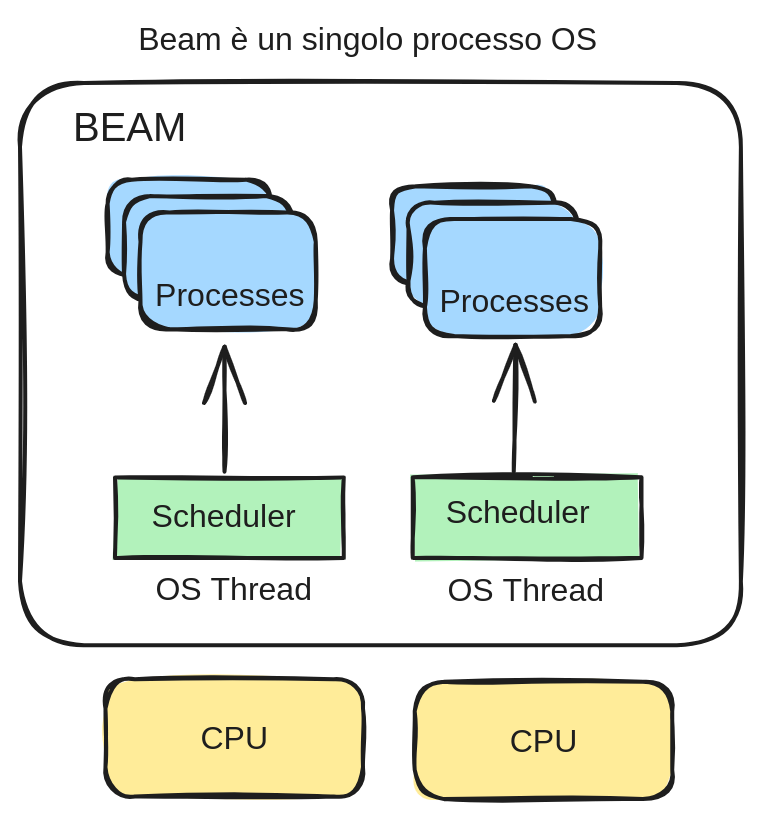
\includegraphics[keepaspectratio=true,scale=0.25]{images/beam_concurrency.png}
	\caption{Concorrenza nella VM Beam \cite{elixirInAction5}}
  	\label{fig:concorrenza_beam}
\end{figure}


%--------------------------------------------------------------

\subsection{Concorrenza basata su attori}

Elixir usa un modello di concorrenza basato su attori,
gli attori sono entità di elaborazione indipendenti
che eseguono operazioni in modo asincrono, questi attori
non sono altro che processi che vengono identificati
attraverso un \textbf{PID} univoco. Come già detto
sono isolati l'uno dall'altro e
comunicano solo attraverso lo scambio di messaggi,
questo scambio avviene attraverso
dei canali di comunicazione detti \textbf{"mailbox"}.
Ogni processo ha una propria mailbox dove avviene la
ricezione del messaggio da parte di altri processi.

I processi sono identificati da un PID univoco,
e conoscendo il PID di un processo può avvenire la comunicazione
attraverso la primitiva fornita dal linguaggio \textbf{send/2}
che permette di inviare un messaggio ad un processo
come avviene nell'esempio \ref{lst:memoryoneprocess}, dove
il processo principale crea un altro processo che rimane in ascolto
tramite il blocco \textbf{receive/1}.
Quest'ultimo quando riceve il messaggio di \textbf{:stop}
viene terminato concludendo il flusso definito dal processo.

Se non ci sono messaggi nella mailbox, il processo aspetta fino a
quando non arriva un messaggio, in particolare, 
nell'esempio tutti i messaggi che
non siano :stop, verranno ignorati continuando ad ascoltare altri
messaggi chiamando ricorsivamente se stesso.

\subsubsection{Process Linking e Process monitoring}

I processi sono isolati, ma si può legare un processo
al processo chiamante tramite un operazione di Process linking,
questo per sapere se il processo va in errore
oppure termina per un comportamento imprevisto,
legando i processi si può propagare l'errore nel caso
uno dei due processi non ha senso di esistere preso da solo.

Spesso i processi vengono legati ad un Supervisor, che
lascerà andare in errore i processi figli, e si occuperà
semplicemente di riavviarli seguendo una strategia scelta.
Questa è la filosofia "Let it Crash"
di Erlang, che si contrappone alla gestione delle eccezioni
di altri linguaggi. Si veda l'esempio \ref{lst:processlinking}.

\newpage

\begin{lstlisting}[language=elixir, caption={Process linking},captionpos=b,
	label={lst:processlinking}]
iex(1)>spawn(fn -> raise "oops" end)
#PID<0.58.0>
	
[error] Process #PID<0.58.00> raised an exception
** (RuntimeError) oops
	(stdlib) erl_eval.erl:668: :erl_eval.do_apply/6

iex(2)spawn_link(fn -> raise "ooops" end)

17:37:50.425 [error] Process #PID<0.113.0> raised an exception
** (RuntimeError) ooops
** (EXIT from #PID<0.110.0>) shell process 
** exited with reason: {%RuntimeError{message: "ooops"}, []}

iex(2)
\end{lstlisting}

Notiamo nell'esempio \ref{lst:processlinking} che con il comando
la funzione spawn\_link/1 il processo va in errore e propaga
l'errore all'ambiente interattivo iex, riavviando anche
l'ambiente iex.

Nel caso invece non si vuole propagare l'errore al processo
chiamante, si può usare il monitoring tramite la primitiva
spawn\_monitor, in questo caso il processo chiamante
non va in errore insieme al processo chiamato, ma riceve
un messaggio di :DOWN nella mailbox da poter gestire a piacimento.

Si nota in conclusione al paragrafo che è possibile
gestire migliaia di processi molto facilmente senza
incrementare in modo considerevole le risorse in memoria grazie
ai processi leggeri, permettendo
di sviluppare un software orientanto alla concorrenza,
tutto è facilitato dall'isolamento di ogni processo che 
permette di non preoccuparsi di meccanismi di locking e sincronizzazine.
Elixir permette di non preoccuparci di come scalare
le risorse hardware, potendo dare responsabilità ad altri
processi creando più flussi di esecuzione.
\section{OTP - Open Telecom Platform}

L'OTP (Open Telecom Platform) è stato sviluppato
da Ericsson negli anni '80 come insieme di strumenti,
librerie e standard per affrontare le sfide specifiche
del settore delle telecomunicazioni,
come l'affidabilità e la tolleranza agli errori.

Basato sul linguaggio di programmazione Erlang,
OTP è stato progettato per gestire la concorrenza
e le comunicazioni asincrone,
rendendolo ideale per sistemi distribuiti.
Nel corso degli anni, l'OTP ha trovato applicazioni
anche in altri settori, diventando una scelta popolare
per sistemi altamente affidabili e scalabili.

Elixir fornisce un'interfaccia più moderna e una sintassi
più chiara rispetto ad Erlang, mantenendo al tempo stesso
la potenza e l'affidabilità di Erlang e OTP.

Per quanto riguarda il mentanimento di uno
stato, in Elixir si può fare affidamento ai Behaviour
Agent e GenServer, consentendo di dare la responsabilità
al mantenimento di uno stato ad un altro processo.

ci consentono di mantenere uno stato senza dover reinventare la
ruota nello scrivere un modulo soltanto per farlo.
L'approccio nella programmazione è totalmente differente
e piuttosto singolare rispetto ai più comuni linguaggi di programmazione,
ma è proprio questa singolarità che può porta il linguaggio
ad essere orientato alla concorrenza. 

%---------------------------------------------------------------------------------

\subsection{GenServer}
Per mantenere uno stato si potrebbe scrivere un modulo che
tramite le primitive concorrenziali gestiscono lo stato
a piacimento. Elixir però mette a disposizione il Behaviour
GenServer, un OTP server è un modulo con il
"Behaviour" GenServer.
Il "Behaviour" è un meccanismo che consente di definire
uno schema comune per un tipo specifico di processo.

Ad esempio il GenServer Behaviour definisce le funzioni e
le interfacce necessarie per creare un processo server in grado
di gestire le richieste in modo asincrono.
Utilizzando il GenServer Behaviour, è possibile definire i comportamenti
di base del server e personalizzarli secondo le esigenze specifiche
dell'applicazione. 
Questo fornisce un alto livello di astrazione per la gestione
dei processi e semplifica lo sviluppo di sistemi concorrenti e
distribuiti in Elixir.

Il vantaggio di utilizzare un GenServer è che ha un'insieme
di interfacce standard e include funzionalità di tracciamento
e segnalazione degli errori. Si può anche mettere dentro un
albero di supervisione.

Questo Behaviour astrae l'interazione Client-server, come si può vedere
in figura \ref{fig:client_server}  \cite{GenServe6:online},
lo stato è gestito dal Server, e i processi client sono quelli che
devono modificare lo stato o accedere ad esso.

\begin{figure}[!htp]
    \centering
    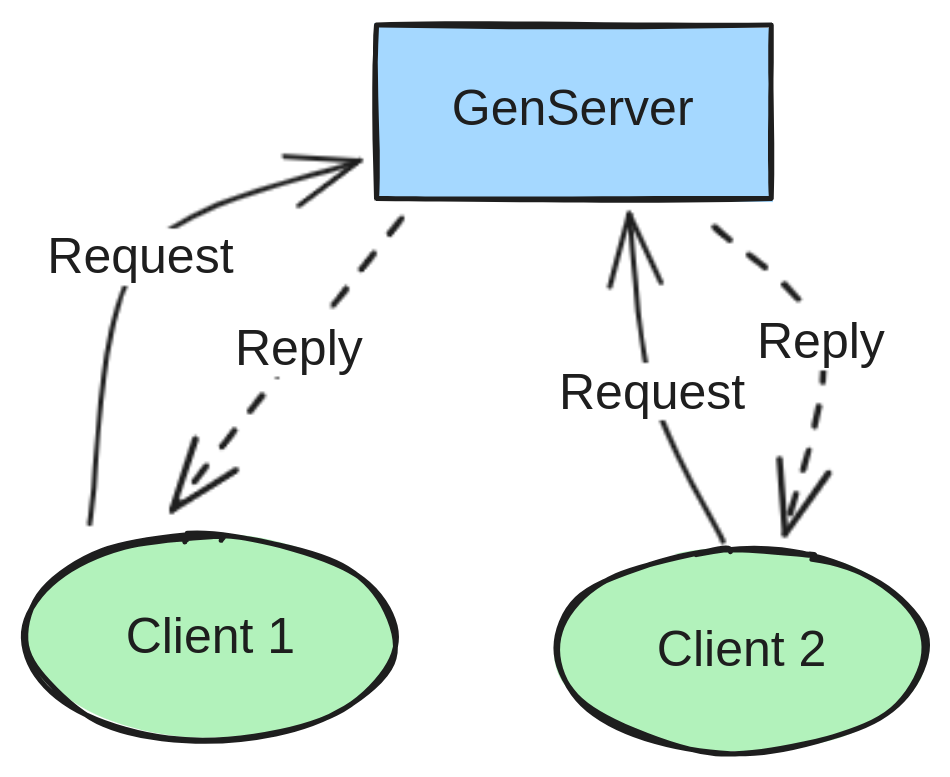
\includegraphics[keepaspectratio=true,scale=0.20]{images/GenServer.png}
	\caption{Interazione Client-Server}
  	\label{fig:client_server}
\end{figure}

Per implementare il behaviour GenServer, bisogna affidarsi alla
documentazione di GenServer, in particolare vanno ridefinite delle
callback, ed ogni funzione può restituire un determinato insieme di
strutture dati.

Nell'esempio \ref{lst:stackGenServer} viene implementata una struttura dati
per mantere uno Stack di dati \cite{GenServe6:online}.

\begin{lstlisting}[language=elixir, caption={Implementazione Stack},captionpos=b,
	label={lst:stackGenServer}]
defmodule Stack do
use GenServer

# Client

def start_link(default) when is_binary(default) do
  GenServer.start_link(__MODULE__, default)
end

def push(pid, element) do
  GenServer.cast(pid, {:push, element})
end

def pop(pid) do
  GenServer.call(pid, :pop)
end

# Server (callbacks)

@impl true
def init(elements) do
  initial_state = String.split(elements, ",", trim: true)
  {:ok, initial_state}
end

@impl true
def handle_call(:pop, _from, state) do
  [to_caller | new_state] = state
  {:reply, to_caller, new_state}
end

@impl true
def handle_cast({:push, element}, state) do
  new_state = [element | state]
  {:noreply, new_state}
end
  end
\end{lstlisting}

Nell'esempio possiamo vedere che il modulo stack implementa
la funzione \textbf{init/1} che inizializza lo stato con gli elementi
iniziali quando il server viene avviato, la funzione \textbf{handle\_call/3}
chiamata per le operazioni di :pop dello stack,
è una funzione sincrona, quindi viene usata quando ci si aspetta
un valore di ritorno, infatti restituisce il valore di
testa dello stack. La funzione \textbf{handle\_cast/2} invece viene usata per
le operazioni asincrone, quindi nel caso in esame per l'operazione di
push nello Stack che non necessita di risposta.

Quindi il GenServer è un'astrazione che:

\begin{itemize}
	\item Incapsula un servizio condiviso.
	\item Mantiene uno stato.
	\item Permette un'astrazione concorrente ad un servizio condiviso \cite{adoptingElixirchap5pag96}.
\end{itemize}

%---------------------------------------------------------------------------------

\subsection{Supervisor}

Un'altro concetto cardine dell'OTP è il Supervisor con cui si
riesce a raggiungere un alto livello di Fault-tolerant.

Il compito principale di un supervisor è quello di monitorare,
controllare e gestire il ciclo di vita dei processi all'interno
di un sistema Erlang o Elixir. I supervisori sono 
particolarmente utili per garantire la stabilità e 
l'affidabilità dei sistemi distribuiti, poiché gestiscono 
automaticamente il riavvio dei processi in caso di fallimenti, 
garantendo che il sistema continui a funzionare anche in
situazioni critiche.

In pratica come il GenServer, un  Supervisor è un modulo
che implementa il Behaviour Supervisor.

\newpage

Ci sono diversi tipi di Supervisor in Erlang ed Elixir, tra cui:
\begin{itemize}
  \item \textbf{Supervisor Semplice}: Questi supervisori monitorano
  direttamente i processi figlio e li riavviano se necessario.
  Sono utilizzati per gestire processi che non hanno stati interni
  o che devono essere riavviati senza alcuna elaborazione specifica.
  \item \textbf{Supervisori gerarchici}: Questi supervisori controllano
  una gerarchia di altri supervisori e processi.
  Possono essere configurati per riavviare solo parti
  specifiche del sistema in caso di problemi,
  consentendo un maggiore controllo sul comportamento di riavvio.
  \item \textbf{Supervisori dinamici}: Questi supervisori possono
  essere creati e configurati dinamicamente durante l'esecuzione
  del programma, consentendo una maggiore flessibilità
  nell'aggiunta e nella gestione dei processi.


 
\end{itemize}

Per implementare un Supervisor di deve decidere quali sono i processi
figli da supervisionare, e si avvia il Supervisor
con la funzione \textbf{start\_link/2}
Bisogna quindi decidere quali sono i processi figli da supervisionare,
e una volta avviato il Supervisor con la funzione \textbf{start\_link/2},
questo ha bisogno di sapere come avviare, fermare o riavviare i suoi figli
in caso di errore o uscita imprevista.

Una volta avviato il Supervisor, deve sapere come fare lo start/stop/restart
dei suoi figli da monitorare. Per questo i moduli da supervisionare
devono implementare una funzione che definisce le specifiche,
la funzione in questione è \textbf{child\_spec/1},
restituisce una Map per
configurare il comportamento in caso di supervisione.

Alcuni moduli come il GenServer già definiscono questa funzione
non avendo la necessità di ridefinirla, come il GenServer e
il modulo Task che utilizzeremo successivamente.

\chapter{Performance - Test sperimentali}

\section{Introduzione}
\chapter*{Conclusioni e sviluppi futuri}
\addcontentsline{toc}{chapter}{Conclusioni e sviluppi futuri}

Elixir si è dimostrato un linguaggio potente che
può migliorare molti aspetti dello sviluppo software,
si è dimostrato di avere uno scheduling molto
veloce che non degrada significamente le performance,
dove non si arriva con Elixir si integrare facilmente
con soluzioni più adatte come il C/C++, Rust o python.
Ha dimostrato di avere una bassa latenza ottimale per
sistemi real time.

Futuri studi possono vedere l'integrazione di Elixir
in software IoT, tramite il framework Nerves o tramite
soluzioni ad Hoc per il caso specifico.


% Capitolo 2




%-------------------------------------------------------------------------
\backmatter

\printbibliography[heading=bibintoc,title={Bibliografia}] % Prints bibliography and display bibliography to toc
\begingroup 
\titleformat{\chapter}
{\normalfont\Huge\bfseries\centering} %shape
{}% label
{} % sep
{}  

\chapter*{Ringraziamenti}


\thispagestyle{empty}



% \shapepar{\heartshape}{\fontfamily{qzc}\fontshape{it}\selectfont{
% Il primo pensiero è per mio fratello Lorenzo, al quale esprimo gratitutidine e al contempo ammirazione per 
% l'eccezionale forza di spirito mostrata dinanzi alle avversità della vita. 
% Sobbarcandosi, come un cireneo, di responsabilità gravose, mi ha consentito di raggiungere la fine di questo percorso.
% Ringrazio mia madre Rita che ha trovato dentro di sè la forza di andare avanti, nonostante tutta l'oscurità.
% Ringrazio, inoltre, i Professori Alessandro Bria e Daniele Pinchera per le parole di stima proferite 
% nei miei confronti a valle dei rispettivi esami che, riecheggiando nella mia mente, mi hanno permesso di andare avanti nei momenti più bui.
% Ringrazio mio zio Giuseppe, per credere sempre in me e nelle mie potenzialità.
% Ringrazio, infine, tutti i miei amici.}}

\endgroup


% N:B IMPORTANT!!!
%\mainmatter gives you normal chapter numbering and arabic page numbering.
%\frontmatter gives you UNNUMBERED chapters (so chapter* is redundant) and roman page numbering.
%\backmatter gives you UNNUMBERED chapters (so chapter* is redundant) and arabic page numbering.


\end{document}